\section{Getting starting with GIMME-2 board }
\label{GIMME2}
In order to interact with the GIMME-2 board the user will need some equipment for the initialization of the GIMME-2 board:

\begin{itemize}
\item Micro-USB Male (Type B) to USB Male (Type A) connector or an Ethernet cable.
\item Power supply, the board should be powered with voltages from range +12V to +24V.
\item The operating system on the machine host is preferred to be Ubuntu 12.04.
\item A serial terminal like gtkterm is needed if the user use a USB cable.
\end{itemize}

Assuming that the GIMME-2 board already has an installed Linux on it the user can interact with the board either through the serial interface (usb cable) or through SSH interface. The user needs to make sure that the jumper on the GIMME-2 board is 0100 before powering on the board.

\subsection{Using serial interface }
Connect the micro-USB to USB connector to the port labelled USB0 on the board and connect the other end to the host PC. Set the voltage of the power supply to +12V and connect it to the GIMME-2 board. Now open the serial terminal and the booting steps can be seen there. Once the booting is over, the user gets a  prompt on the screen.


\subsection{Using Ethernet }
Connect one end of the Ethernet cable to the middle port among the three on the GIMME-2 board and the other end to the host machine. Now open the bash terminal and execute ssh root@192.168.1.10. Type in (root) when password is prompted. The user gets a zynq> prompt on the screen.

Assuming that the user needs to do changes on the ramdisk image on the GIMME-2 board, the user will need to install the full package of Xilinx ISE Design Suite including the software development Kit(SDK) on the host Pc.
Using SDK a new boot image can be created .if the user made some changes on the ramdisk image the user will need to create a new bootable image. 

\subsection{Install operating system on GIMME-2}
For building the boot image from sources refer the Xilinx Wiki . The necessary files for creating a boot file for Linux on the GIMME-2 board is available on the Naiad’s Dropbox. If the root file system needs to be edited please follow the steps in section  \ref{Modifying_the_root_file_system} . For building the latest kernel version, follow the steps section  \ref{Build_Kernel}. The steps to make a bootable image for flash memory using the files in Naiad’s Dropbox are described in section  \ref{Make_a_Linux_Bootable_Image_for_QSPI_Flashl}. Section \ref{Programming_the_QSPI_flash_through_JTAG} describes how to program the flash memory through a JTAG interface.

\subsection{Installing Platform USB Cable II drivers}
For Windows users, no need to install the drivers as it comes with the package of Xilinx ISE Design Suite or Vivado.

For Linux users, first download and install Xilinx ISE Design Suite \cite{XilinxDesign} or Vivado \cite{Vivado}.
The installation process is guided using a GUI like in Windows.

Download the driver from \cite{USBDriver}

Build the library by calling `make'. If you are on a 64 bit system but want to build a 32 bit library, run `make lib32' instead. Be sure to have the 32 bit versions of libusb-devel and libftdi-devel installed.

To use the device as an ordinary user, put the following line in a new file "libusb-driver.rules" in /etc/udev/rules.d/  

ACTION=="add", SUBSYSTEMS=="usb", ATTRS{idVendor}=="03fd", MODE="666"
and restart udev.

If your cable does not have the ID 03fd:0008 in the output of lsusb, the initial firmware has not been loaded (loading it changes the
product-ID from another value to 8). To load the firmware follow these steps:

Run ./setup\_pcusb in this directory, this should set up everything correctly: \\
   When XILINX is set correctly: \\
      ./setup\_pcusb \\
    When XILINX is not set, and ISE is installed in /opt/Xilinx/14.7: \\
      ./setup\_pcusb /opt/Xilinx/14.7/ISE\_DS/ISE 

\subsection{Modifying the root file system} 
\label{Modifying_the_root_file_system}
Initrd and initramfs refer to two different methods for loading a temporary root file system into memory in the boot process of Linux kernel. For GIMME-2 board, we have a prebuilt initrd and initramfs image from Xilinx\cite{xilinxwiki}.

\subsection{Modify an initial ramdisk of type initrd}
Assuming that your image called (ramdisk.image.gz): 
\begin{enumerate}
\item Unwrap the wrapped image.
\begin{lstlisting}[language=bash]
$ dd if=./uramdisk.image.gz bs=64 skip=1 of=ramdisk.image.gz 
\end{lstlisting}
\item Extract the initrd image from the gzip archive.
\begin{lstlisting}[language=bash]
$ gunzip ramdisk.image.gz 
\end{lstlisting}
\item Mount the initrd image.
\begin{lstlisting}[language=bash]
$ chmod u+rwx ramdisk.image 
$ mkdir tmp_mnt/ 
$ sudo mount -o loop ramdisk.image tmp_mnt/ 
\end{lstlisting}
\item Make changes in the mounted filesystem if required. Otherwise skip to step 5.
\begin{lstlisting}[language=bash]
$ cd etc/init.d/ 
$ sudo gedit rcS 
\end{lstlisting}
\item Go to folder location where tmp\_mnt resides. Unmount the initrd image and compress the image.
\begin{lstlisting}[language=bash]
$ sudo umount tmp_mnt/ 
$ gzip ramdisk.image 
\end{lstlisting}
\item ramdisk.image.gz needs to be wrapped with a U-Boot header in order for U-Boot boot with it:
\begin{lstlisting}[language=bash]
$ mkimage -A arm -T ramdisk -C gzip -d ramdisk.image.gz uramdisk.image.gz.
\end{lstlisting}
\end{enumerate}
\subsection{Modify an initial ramdisk of type initramfs}

Assuming that your image called (ramdisk.image.gz):
\begin{enumerate}
\item Create a temporary folder
\begin{lstlisting}[language=bash]
$ sudo mkdir /tmp/rootfs 
\end{lstlisting}
\item Unwrap the wrapped image.
\begin{lstlisting}[language=bash]
$ sudo dd if=uramdisk.image.gz of=ramdisk.image.gz bs=64 skip=1 
\end{lstlisting}
\item Extract the initramfs image from the gzip archive and mount it.
\begin{lstlisting}[language=bash]
$ sudo gunzip -c ramdisk.image.gz | sudo sh -c 'cd /tmp/rootfs/ && cpio -i' 
\end{lstlisting}
\item Go to /tmp/rootfs/ and make the changes in the file systems if required.
\item Unmount the initramfs image and compress the image.
\begin{lstlisting}[language=bash]
$ sudo sh -c 'cd /tmp/rootfs/ && sudo find . 
    | sudo cpio -H newc -o' | gzip -9 > ramdisk.image.gz 
\end{lstlisting}
\item ramdisk.image.gz needs to be wrapped with a U-Boot header in order for U-Boot boot with it:
\begin{lstlisting}[language=bash]
$ sudo mkimage -A arm -T ramdisk -C gzip -d ramdisk.image.gz uramdisk.image.gz 
\end{lstlisting}
\item Delete the temporary folder and old ramdisk image:
\begin{lstlisting}[language=bash]
$ sudo rm ramdisk.image.gz 
$ sudo rm -rf /tmp/rootfs 
\end{lstlisting}
\end{enumerate}
\subsection{Build Kernel}
\label{Build_Kernel}

\begin{lstlisting}[language=bash]
$ make ARCH=arm xilinx_zynq_defconfig 
$ make ARCH=arm menuconfig 
\end{lstlisting}
To produce the kernel image:
\begin{lstlisting}[language=bash]
$ make ARCH=arm UIMAGE_LOADADDR=0x8000 uImage 
$ CROSS\_COMPILE=/opt/Xilinx/14.6/ISE_DS/ -EDK/gnu/arm/lin/bin/arm-xilinx-linux-gnueabi
\end{lstlisting}
\subsection{Make a Linux Bootable Image for QSPI Flash}
\label{Make_a_Linux_Bootable_Image_for_QSPI_Flashl}
\begin{enumerate}
\item In SDK, select Xilinx Tools > Create Zynq Boot Image. The Create Zynq Boot Image wizard opens. 
\item Add the necessary files as shown in the figure and give the offsets(offsets can be changed depending on the GIMME-2 board):\newline
 \makebox[\paperwidth][l]{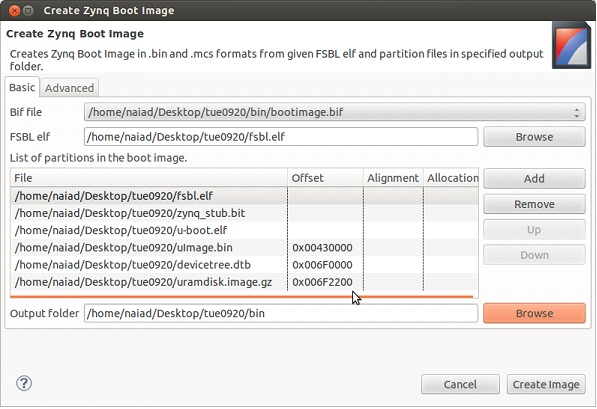
\includegraphics[height=6cm]{./Images/GIMME-2/1}}

\item Click Create Image. \\
The Create Zynq Boot Image window creates following files in the specified output folder: \\
 bootimage.bif \\
 u-boot.bin
\end{enumerate}
\subsection{Programming the QSPI flash through JTAG}
\label{Programming_the_QSPI_flash_through_JTAG}
Requirements:
\begin{itemize}
\item XILINX Platform USB Cable II (JTAG interface)
\item micro-USB cable OR Ethernet cable
\item Xilinx SDK 
\end{itemize}
\begin{enumerate}

\item Set boot jumpers for JTAG-boot - 0000 - and power up the board (the boot jumpers are on the GIMME-2 board) \newline
 \makebox[\paperwidth][l]{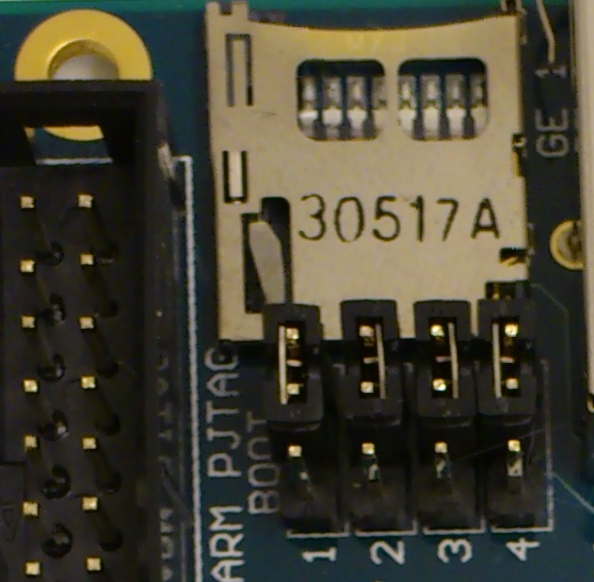
\includegraphics[ height=5cm]{./Images/GIMME-2/jtag0000}}

\item Program the FPGA - gimme\_top.bit. 
\item Start terminal (Prefered to used GtkTerm) and set the following configuration: 

 \makebox[\paperwidth][l]{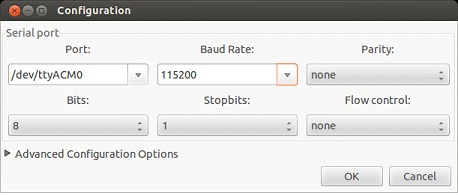
\includegraphics[height=4cm]{./Images/GIMME-2/2}}

\item In SDK, start console (Xilinx Tools -> XMD Console) . Execute these commands:
\begin{lstlisting}[language=bash]
$ connect arm hw 
$ source <path>/ps7_init.tcl 
$ ps7_init 
$ ps7_post_config  
$ dow <path>/u-boot.elf 
$ dow -data <path>/u-boot.bin 0x08000000 
$ con 
\end{lstlisting}
\item As soon as you enter “con” in XMD console, switch to serial terminal. 
\item In terminal, stop autoboot when it shows - "Hit any key to stop autoboot: 3" and enter these commands: 
\begin{lstlisting}[language=bash]
$ sf probe 0 0 0 
$ sf erase 0 0x01000000 
$ sf write 0x08000000 0 0xFFFFFF 
\end{lstlisting}
\item Power off board, set boot jumpers for QSPI-boot - 0100 - Power on board \newline
 \makebox[\paperwidth][l]{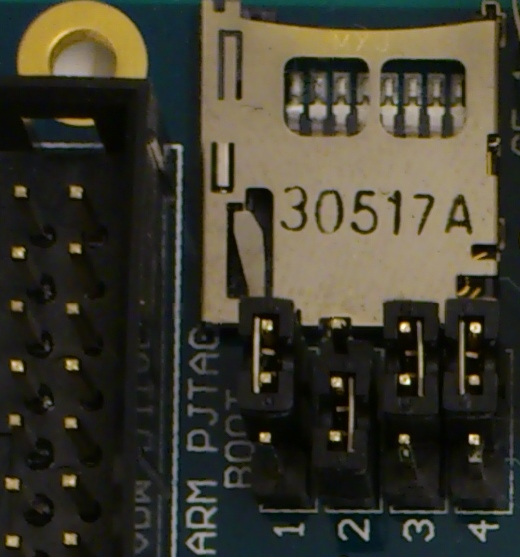
\includegraphics[width=6cm]{./Images/GIMME-2/jtag0100}}
\item Start terminal or connect on ssh 192.168.1.10 u: root, p: root
\end{enumerate}
\begin{thebibliography}{99}
\bibitem{XilinxDesign}
http://www.xilinx.com/support/download/index.html/content/xilinx/en/downloadNav/design-tools.html,date,2014-09-15  
\bibitem{Vivado}
http://www.xilinx.com/support/download/index.html/content/xilinx/en/downloadNav/vivado-design-tools.html,date,2014-09-25 
\bibitem{USBDriver}
http://git.zerfleddert.de/cgi-bin/gitweb.cgi/usb-driver?a=snapshot;h=HEAD;sf=tgz,date,2014-09-10
\bibitem{xilinxwiki}
http://www.wiki.xilinx.com/Zynq+Releases,date,2014-09-15 
\end{thebibliography}